\documentclass[twoside]{book}

% Packages required by doxygen
\usepackage{fixltx2e}
\usepackage{calc}
\usepackage{doxygen}
\usepackage[export]{adjustbox} % also loads graphicx
\usepackage{graphicx}
\usepackage[utf8]{inputenc}
\usepackage{makeidx}
\usepackage{multicol}
\usepackage{multirow}
\PassOptionsToPackage{warn}{textcomp}
\usepackage{textcomp}
\usepackage[nointegrals]{wasysym}
\usepackage[table]{xcolor}

% Font selection
\usepackage[T1]{fontenc}
\usepackage[scaled=.90]{helvet}
\usepackage{courier}
\usepackage{amssymb}
\usepackage{sectsty}
\renewcommand{\familydefault}{\sfdefault}
\allsectionsfont{%
  \fontseries{bc}\selectfont%
  \color{darkgray}%
}
\renewcommand{\DoxyLabelFont}{%
  \fontseries{bc}\selectfont%
  \color{darkgray}%
}
\newcommand{\+}{\discretionary{\mbox{\scriptsize$\hookleftarrow$}}{}{}}

% Page & text layout
\usepackage{geometry}
\geometry{%
  a4paper,%
  top=2.5cm,%
  bottom=2.5cm,%
  left=2.5cm,%
  right=2.5cm%
}
\tolerance=750
\hfuzz=15pt
\hbadness=750
\setlength{\emergencystretch}{15pt}
\setlength{\parindent}{0cm}
\setlength{\parskip}{3ex plus 2ex minus 2ex}
\makeatletter
\renewcommand{\paragraph}{%
  \@startsection{paragraph}{4}{0ex}{-1.0ex}{1.0ex}{%
    \normalfont\normalsize\bfseries\SS@parafont%
  }%
}
\renewcommand{\subparagraph}{%
  \@startsection{subparagraph}{5}{0ex}{-1.0ex}{1.0ex}{%
    \normalfont\normalsize\bfseries\SS@subparafont%
  }%
}
\makeatother

% Headers & footers
\usepackage{fancyhdr}
\pagestyle{fancyplain}
\fancyhead[LE]{\fancyplain{}{\bfseries\thepage}}
\fancyhead[CE]{\fancyplain{}{}}
\fancyhead[RE]{\fancyplain{}{\bfseries\leftmark}}
\fancyhead[LO]{\fancyplain{}{\bfseries\rightmark}}
\fancyhead[CO]{\fancyplain{}{}}
\fancyhead[RO]{\fancyplain{}{\bfseries\thepage}}
\fancyfoot[LE]{\fancyplain{}{}}
\fancyfoot[CE]{\fancyplain{}{}}
\fancyfoot[RE]{\fancyplain{}{\bfseries\scriptsize Generated by Doxygen }}
\fancyfoot[LO]{\fancyplain{}{\bfseries\scriptsize Generated by Doxygen }}
\fancyfoot[CO]{\fancyplain{}{}}
\fancyfoot[RO]{\fancyplain{}{}}
\renewcommand{\footrulewidth}{0.4pt}
\renewcommand{\chaptermark}[1]{%
  \markboth{#1}{}%
}
\renewcommand{\sectionmark}[1]{%
  \markright{\thesection\ #1}%
}

% Indices & bibliography
\usepackage{natbib}
\usepackage[titles]{tocloft}
\setcounter{tocdepth}{3}
\setcounter{secnumdepth}{5}
\makeindex

% Hyperlinks (required, but should be loaded last)
\usepackage{ifpdf}
\ifpdf
  \usepackage[pdftex,pagebackref=true]{hyperref}
\else
  \usepackage[ps2pdf,pagebackref=true]{hyperref}
\fi
\hypersetup{%
  colorlinks=true,%
  linkcolor=blue,%
  citecolor=blue,%
  unicode%
}

% Custom commands
\newcommand{\clearemptydoublepage}{%
  \newpage{\pagestyle{empty}\cleardoublepage}%
}

\usepackage{caption}
\captionsetup{labelsep=space,justification=centering,font={bf},singlelinecheck=off,skip=4pt,position=top}

%===== C O N T E N T S =====

\begin{document}

% Titlepage & ToC
\hypersetup{pageanchor=false,
             bookmarksnumbered=true,
             pdfencoding=unicode
            }
\pagenumbering{roman}
\begin{titlepage}
\vspace*{7cm}
\begin{center}%
{\Large Heisprosjekt -\/ Gruppe 10 }\\
\vspace*{1cm}
{\large Generated by Doxygen 1.8.11}\\
\end{center}
\end{titlepage}
\clearemptydoublepage
\tableofcontents
\clearemptydoublepage
\pagenumbering{arabic}
\hypersetup{pageanchor=true}

%--- Begin generated contents ---
\chapter{Elevator project -\/ T\+T\+K4235 -\/ Group 10}
\label{index}\hypertarget{index}{}\hypertarget{index_intro_sec}{}\section{Introduction}\label{index_intro_sec}
This page contains the documentation for our elevator project.\hypertarget{index_summary}{}\section{Implementation summary}\label{index_summary}
\hypertarget{index_fsm}{}\subsection{Finite State Machine (\+F\+S\+M)}\label{index_fsm}
Our elevator implementation is based on a finite state machine. All states in the F\+SM is in itself its own function and thus the current state is simply determined by which function is called. Each function returns a return code which is part of determining the next state function to call. The F\+SM includes a transition table which contains all possible state transitions and a lookup function. This lookup function uses the transition table to find the next state based on the current state and the return code given by the current state function. In the main loop inside the main function in \hyperlink{main_8c_source}{main.\+c} the state is then updated and the next state function is called. The F\+SM is implemented in the \hyperlink{fsm_8c_source}{fsm.\+c} file.\hypertarget{index_exec}{}\subsection{Execution handler}\label{index_exec}
This project also has an execution handler module which is responsible for the actions of the elevator. The thought here is that the state functions in the F\+SM mostly just calls function in the execution handler to handle orders, get return codes, etc. The execution handler is implemented in the \hyperlink{exec_8c_source}{exec.\+c} file.\hypertarget{index_order_and_scheduler}{}\subsection{Order handling system}\label{index_order_and_scheduler}
The order handling system is based around two queues, one for orders made inside the elevator and one for orders made outside the elevator. The reason for the seperation is because we believe that orders made inside the elevator should be executed before orders made outside the elevator, and thus having two seperate queues eases the logic for deciding which order to handle. To handle these queues our A\+PI includes a scheduler and an order handler.\hypertarget{index_scheduler}{}\subsubsection{Scheduler}\label{index_scheduler}
The scheduler handles the queue specific tasks of adding and deleting orders. It is based on a first in, first out principle to prioritize the orders. The scheduler also handles all the logic of validating the orders. This validation is specific for this elevator. The scheduler is implemented in the \hyperlink{scheduler_8c_source}{scheduler.\+c} file.\hypertarget{index_order}{}\subsubsection{Order handler}\label{index_order}
The order handler serves as a link between the execution handler and the scheduler and does most of the ordering tasks, specific to this elevator such as removing all orders at all floor. The reasoning for this is to get another level of abstraction in the queue system. The implementation of the order handler can be found in the \hyperlink{order_8c_source}{order.\+c} file. 
\chapter{Data Structure Index}
\section{Data Structures}
Here are the data structures with brief descriptions\+:\begin{DoxyCompactList}
\item\contentsline{section}{\hyperlink{structinside__order}{inside\+\_\+order} }{\pageref{structinside__order}}{}
\item\contentsline{section}{\hyperlink{structinside__order__queue}{inside\+\_\+order\+\_\+queue} }{\pageref{structinside__order__queue}}{}
\item\contentsline{section}{\hyperlink{structoutside__order}{outside\+\_\+order} }{\pageref{structoutside__order}}{}
\item\contentsline{section}{\hyperlink{structoutside__order__queue}{outside\+\_\+order\+\_\+queue} }{\pageref{structoutside__order__queue}}{}
\item\contentsline{section}{\hyperlink{structtransition}{transition} }{\pageref{structtransition}}{}
\end{DoxyCompactList}

\chapter{File Index}
\section{File List}
Here is a list of all documented files with brief descriptions\+:\begin{DoxyCompactList}
\item\contentsline{section}{source/{\bfseries channels.\+h} }{\pageref{channels_8h}}{}
\item\contentsline{section}{source/{\bfseries elev.\+c} }{\pageref{elev_8c}}{}
\item\contentsline{section}{source/{\bfseries elev.\+h} }{\pageref{elev_8h}}{}
\item\contentsline{section}{source/{\bfseries exec.\+c} }{\pageref{exec_8c}}{}
\item\contentsline{section}{source/\hyperlink{exec_8h}{exec.\+h} \\*A library for executing tasks for the elevator }{\pageref{exec_8h}}{}
\item\contentsline{section}{source/{\bfseries fsm.\+c} }{\pageref{fsm_8c}}{}
\item\contentsline{section}{source/\hyperlink{fsm_8h}{fsm.\+h} \\*A state machine library }{\pageref{fsm_8h}}{}
\item\contentsline{section}{source/{\bfseries io.\+c} }{\pageref{io_8c}}{}
\item\contentsline{section}{source/{\bfseries io.\+h} }{\pageref{io_8h}}{}
\item\contentsline{section}{source/{\bfseries main.\+c} }{\pageref{main_8c}}{}
\item\contentsline{section}{source/{\bfseries order.\+c} }{\pageref{order_8c}}{}
\item\contentsline{section}{source/\hyperlink{order_8h}{order.\+h} \\*A library for order and queue tasks specific to this elevator }{\pageref{order_8h}}{}
\item\contentsline{section}{source/{\bfseries scheduler.\+c} }{\pageref{scheduler_8c}}{}
\item\contentsline{section}{source/\hyperlink{scheduler_8h}{scheduler.\+h} \\*A library for doing operations on queues }{\pageref{scheduler_8h}}{}
\end{DoxyCompactList}

\chapter{Data Structure Documentation}
\hypertarget{structinside__order}{}\section{inside\+\_\+order Struct Reference}
\label{structinside__order}\index{inside\+\_\+order@{inside\+\_\+order}}
\subsection*{Data Fields}
\begin{DoxyCompactItemize}
\item 
floor\+\_\+codes\+\_\+t {\bfseries floor}\hypertarget{structinside__order_a5f816e91e84a8bd27ac2a179c43691dc}{}\label{structinside__order_a5f816e91e84a8bd27ac2a179c43691dc}

\end{DoxyCompactItemize}


\subsection{Detailed Description}


Definition at line 27 of file scheduler.\+h.



The documentation for this struct was generated from the following file\+:\begin{DoxyCompactItemize}
\item 
source/\hyperlink{scheduler_8h}{scheduler.\+h}\end{DoxyCompactItemize}

\hypertarget{structinside__order__queue}{}\section{inside\+\_\+order\+\_\+queue Struct Reference}
\label{structinside__order__queue}\index{inside\+\_\+order\+\_\+queue@{inside\+\_\+order\+\_\+queue}}


Collaboration diagram for inside\+\_\+order\+\_\+queue\+:\nopagebreak
\begin{figure}[H]
\begin{center}
\leavevmode
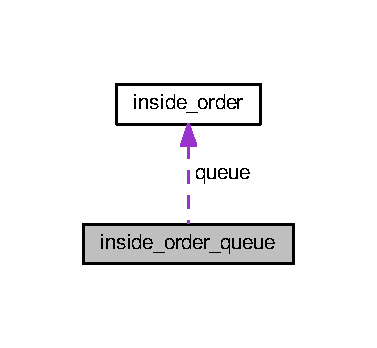
\includegraphics[width=181pt]{structinside__order__queue__coll__graph}
\end{center}
\end{figure}
\subsection*{Data Fields}
\begin{DoxyCompactItemize}
\item 
int {\bfseries length}\hypertarget{structinside__order__queue_af25818967b7fcb1153ca2f3b0680526f}{}\label{structinside__order__queue_af25818967b7fcb1153ca2f3b0680526f}

\item 
int {\bfseries rear}\hypertarget{structinside__order__queue_ab8e16f2ab4d7e5563e98981b4f5f0d54}{}\label{structinside__order__queue_ab8e16f2ab4d7e5563e98981b4f5f0d54}

\item 
\hyperlink{structinside__order}{inside\+\_\+order\+\_\+t} {\bfseries queue} \mbox{[}M\+A\+X\+\_\+\+I\+N\+S\+I\+D\+E\+\_\+\+O\+R\+D\+E\+RS\mbox{]}\hypertarget{structinside__order__queue_a4dd512cf1ce8c0f4d5ff0b8cacbfc6cd}{}\label{structinside__order__queue_a4dd512cf1ce8c0f4d5ff0b8cacbfc6cd}

\end{DoxyCompactItemize}


\subsection{Detailed Description}


Definition at line 36 of file scheduler.\+h.



The documentation for this struct was generated from the following file\+:\begin{DoxyCompactItemize}
\item 
source/\hyperlink{scheduler_8h}{scheduler.\+h}\end{DoxyCompactItemize}

\hypertarget{structoutside__order}{}\section{outside\+\_\+order Struct Reference}
\label{structoutside__order}\index{outside\+\_\+order@{outside\+\_\+order}}
\subsection*{Data Fields}
\begin{DoxyCompactItemize}
\item 
floor\+\_\+codes\+\_\+t {\bfseries floor}\hypertarget{structoutside__order_a46a26592b06dc0c6c95462014a8087c2}{}\label{structoutside__order_a46a26592b06dc0c6c95462014a8087c2}

\item 
elev\+\_\+motor\+\_\+direction\+\_\+t {\bfseries direction}\hypertarget{structoutside__order_a542a2b3f86ab377e9cff750de95e1fe3}{}\label{structoutside__order_a542a2b3f86ab377e9cff750de95e1fe3}

\end{DoxyCompactItemize}


\subsection{Detailed Description}


Definition at line 31 of file scheduler.\+h.



The documentation for this struct was generated from the following file\+:\begin{DoxyCompactItemize}
\item 
source/\hyperlink{scheduler_8h}{scheduler.\+h}\end{DoxyCompactItemize}

\hypertarget{structoutside__order__queue}{}\section{outside\+\_\+order\+\_\+queue Struct Reference}
\label{structoutside__order__queue}\index{outside\+\_\+order\+\_\+queue@{outside\+\_\+order\+\_\+queue}}


Collaboration diagram for outside\+\_\+order\+\_\+queue\+:\nopagebreak
\begin{figure}[H]
\begin{center}
\leavevmode
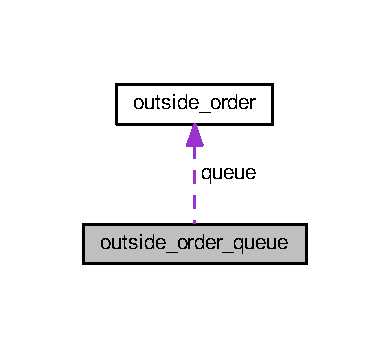
\includegraphics[width=187pt]{structoutside__order__queue__coll__graph}
\end{center}
\end{figure}
\subsection*{Data Fields}
\begin{DoxyCompactItemize}
\item 
int {\bfseries length}\hypertarget{structoutside__order__queue_a8259fe8daf9f79a1acb9523b5750bd77}{}\label{structoutside__order__queue_a8259fe8daf9f79a1acb9523b5750bd77}

\item 
int {\bfseries rear}\hypertarget{structoutside__order__queue_af5116728b6d122a7b020ed4bd1a32f1b}{}\label{structoutside__order__queue_af5116728b6d122a7b020ed4bd1a32f1b}

\item 
\hyperlink{structoutside__order}{outside\+\_\+order\+\_\+t} {\bfseries queue} \mbox{[}M\+A\+X\+\_\+\+O\+U\+T\+S\+I\+D\+E\+\_\+\+O\+R\+D\+E\+RS\mbox{]}\hypertarget{structoutside__order__queue_a42fc224e7f768fb3b882628d8c052ca4}{}\label{structoutside__order__queue_a42fc224e7f768fb3b882628d8c052ca4}

\end{DoxyCompactItemize}


\subsection{Detailed Description}


Definition at line 53 of file scheduler.\+h.



The documentation for this struct was generated from the following file\+:\begin{DoxyCompactItemize}
\item 
source/\hyperlink{scheduler_8h}{scheduler.\+h}\end{DoxyCompactItemize}

\hypertarget{structtransition}{}\section{transition Struct Reference}
\label{structtransition}\index{transition@{transition}}
\subsection*{Data Fields}
\begin{DoxyCompactItemize}
\item 
state\+\_\+codes\+\_\+t {\bfseries src\+\_\+state}\hypertarget{structtransition_aface180c1b7e268ee434c9345069ef9a}{}\label{structtransition_aface180c1b7e268ee434c9345069ef9a}

\item 
return\+\_\+codes\+\_\+t {\bfseries return\+\_\+code}\hypertarget{structtransition_ae9946d3b2fde2a6af4a08763cbdef682}{}\label{structtransition_ae9946d3b2fde2a6af4a08763cbdef682}

\item 
state\+\_\+codes\+\_\+t {\bfseries destination\+\_\+state}\hypertarget{structtransition_a8e0c6c5a7221b92e8722acdb01627a5f}{}\label{structtransition_a8e0c6c5a7221b92e8722acdb01627a5f}

\end{DoxyCompactItemize}


\subsection{Detailed Description}


Definition at line 44 of file fsm.\+h.



The documentation for this struct was generated from the following file\+:\begin{DoxyCompactItemize}
\item 
source/\hyperlink{fsm_8h}{fsm.\+h}\end{DoxyCompactItemize}

\chapter{File Documentation}
\hypertarget{exec_8h}{}\section{source/exec.h File Reference}
\label{exec_8h}\index{source/exec.\+h@{source/exec.\+h}}


A library for executing tasks for the elevator.  


{\ttfamily \#include \char`\"{}order.\+h\char`\"{}}\\*
Include dependency graph for exec.\+h\+:\nopagebreak
\begin{figure}[H]
\begin{center}
\leavevmode
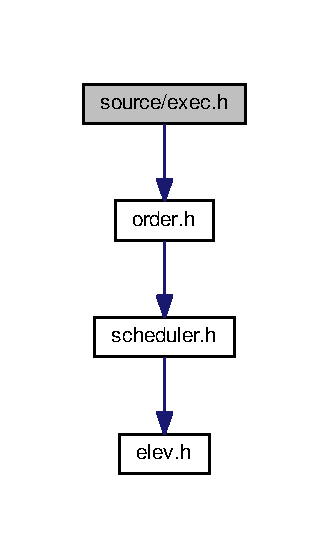
\includegraphics[width=158pt]{exec_8h__incl}
\end{center}
\end{figure}
This graph shows which files directly or indirectly include this file\+:\nopagebreak
\begin{figure}[H]
\begin{center}
\leavevmode
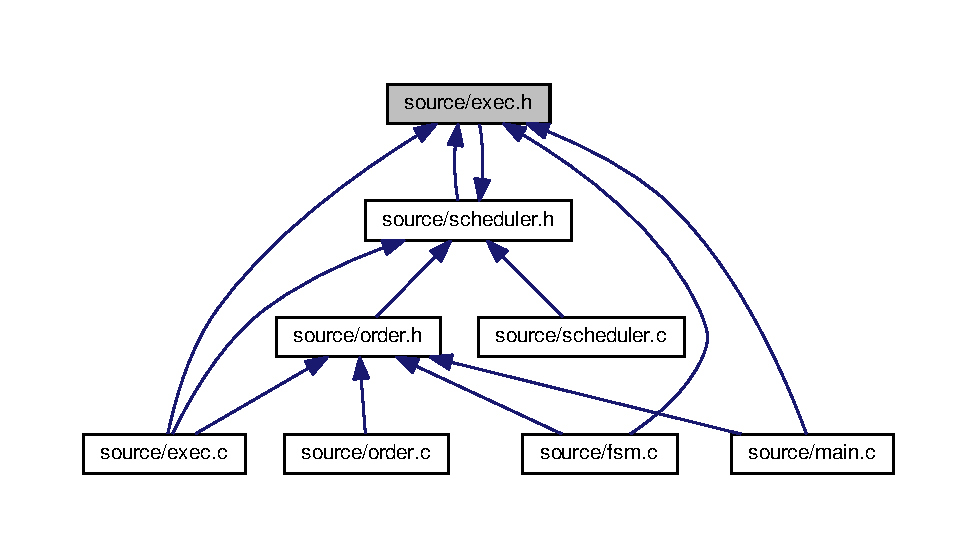
\includegraphics[width=299pt]{exec_8h__dep__incl}
\end{center}
\end{figure}
\subsection*{Typedefs}
\begin{DoxyCompactItemize}
\item 
typedef enum return\+\_\+codes {\bfseries return\+\_\+codes\+\_\+t}\hypertarget{exec_8h_a7e5229089fb5f6f8e34ff43399954f01}{}\label{exec_8h_a7e5229089fb5f6f8e34ff43399954f01}

\end{DoxyCompactItemize}
\subsection*{Enumerations}
\begin{DoxyCompactItemize}
\item 
enum {\bfseries return\+\_\+codes} \{ \\*
{\bfseries drive\+\_\+up}, 
{\bfseries drive\+\_\+down}, 
{\bfseries hold}, 
{\bfseries stay}, 
\\*
{\bfseries idle}, 
{\bfseries stop}, 
{\bfseries fail}
 \}\hypertarget{exec_8h_aaca7161d951febc512af343029761de1}{}\label{exec_8h_aaca7161d951febc512af343029761de1}

\end{DoxyCompactItemize}
\subsection*{Functions}
\begin{DoxyCompactItemize}
\item 
void \hyperlink{exec_8h_a26b32e8c9174585991c50dcab220eff2}{exec\+\_\+delay} (int ms)
\begin{DoxyCompactList}\small\item\em Delay operations for {\ttfamily ms} milliseconds. \end{DoxyCompactList}\item 
void \hyperlink{exec_8h_a0247722e69d060b83c0cc693d7f1bbed}{exec\+\_\+update\+\_\+destination\+\_\+floor} (void)\hypertarget{exec_8h_a0247722e69d060b83c0cc693d7f1bbed}{}\label{exec_8h_a0247722e69d060b83c0cc693d7f1bbed}

\begin{DoxyCompactList}\small\item\em Update the current destination floor found in the private variable {\ttfamily destination\+\_\+floor}. Choose the first element of the inside queue. If the inside queue is empty, choose the first element of the outside queue. If both queues are empty {\ttfamily destination\+\_\+floor} is set to {\ttfamily between\+\_\+floors} to symbolize that the elevator has no orders to handle. \end{DoxyCompactList}\item 
void \hyperlink{exec_8h_ac541593f1c96970ca74a9fbf07e5af72}{exec\+\_\+set\+\_\+last\+\_\+floor} (floor\+\_\+codes\+\_\+t floor)
\begin{DoxyCompactList}\small\item\em Update the private variable {\ttfamily last\+\_\+floor} with the last floor the elevator was at. \end{DoxyCompactList}\item 
void \hyperlink{exec_8h_a187983c2e979e6c1a270225d55b796e3}{exec\+\_\+clear\+\_\+all\+\_\+order\+\_\+lights\+\_\+at\+\_\+floor} (floor\+\_\+codes\+\_\+t floor)
\begin{DoxyCompactList}\small\item\em Turn off all order lamps for a given floor. Both outside and inside order lamps. \end{DoxyCompactList}\item 
void \hyperlink{exec_8h_a04c0ea9caccae0e340032952ead22bd7}{exec\+\_\+set\+\_\+last\+\_\+direction} (elev\+\_\+motor\+\_\+direction\+\_\+t direction)
\begin{DoxyCompactList}\small\item\em Update the private variable {\ttfamily last\+\_\+direction} to the last direction the elevator was moving in. \end{DoxyCompactList}\item 
void \hyperlink{exec_8h_aba63d82da051bcf86283bf21746f72ca}{exec\+\_\+check\+\_\+order\+\_\+buttons} (void)\hypertarget{exec_8h_aba63d82da051bcf86283bf21746f72ca}{}\label{exec_8h_aba63d82da051bcf86283bf21746f72ca}

\begin{DoxyCompactList}\small\item\em Check all order buttons and update inside and outside queues accordingly. Turn on correct order lamp if an order was made. \end{DoxyCompactList}\item 
int \hyperlink{exec_8h_af110d3781ffe6a902da82f19001e458c}{exec\+\_\+should\+\_\+stop\+\_\+at\+\_\+floor} (floor\+\_\+codes\+\_\+t current\+\_\+floor)
\begin{DoxyCompactList}\small\item\em Check if the elevator should stop at a floor. Search both queues for orders. If orders found check if the floor (and direction) of the order matches {\ttfamily current\+\_\+floor} (and {\ttfamily last\+\_\+direction}). \end{DoxyCompactList}\item 
return\+\_\+codes\+\_\+t \hyperlink{exec_8h_a133a405baba27d508f375109e8ced16f}{exec\+\_\+get\+\_\+idle\+\_\+return\+\_\+code} (void)
\begin{DoxyCompactList}\small\item\em Fetch the return code for the idle state. Algorithm for finding the return code is based on the private variables {\ttfamily destination\+\_\+floor}, {\ttfamily last\+\_\+floor} and {\ttfamily last\+\_\+direction}. \end{DoxyCompactList}\item 
return\+\_\+codes\+\_\+t \hyperlink{exec_8h_ac063bc987fc327157be6ca9810167b9c}{exec\+\_\+get\+\_\+floor\+\_\+return\+\_\+code} (floor\+\_\+codes\+\_\+t current\+\_\+floor)
\begin{DoxyCompactList}\small\item\em Fetch the return code for the floor\+\_\+stationary state. The algorithm for finding the return code is based on the private variable {\ttfamily destination\+\_\+floor} and the parameter {\ttfamily current\+\_\+floor}. \end{DoxyCompactList}\item 
return\+\_\+codes\+\_\+t \hyperlink{exec_8h_afc1c4e77dbaa1a140691d21bde08d47b}{exec\+\_\+open\+\_\+door\+\_\+3\+\_\+sec} (floor\+\_\+codes\+\_\+t current\+\_\+floor)
\begin{DoxyCompactList}\small\item\em Open the door for 3 seconds. Check for new orders while door is open and remove orders made for the current floor. Reset timer if a new order is made for the current floor while the door is open. Check if stop button is pressed while the door is open. \end{DoxyCompactList}\end{DoxyCompactItemize}


\subsection{Detailed Description}
A library for executing tasks for the elevator. 



\subsection{Function Documentation}
\index{exec.\+h@{exec.\+h}!exec\+\_\+clear\+\_\+all\+\_\+order\+\_\+lights\+\_\+at\+\_\+floor@{exec\+\_\+clear\+\_\+all\+\_\+order\+\_\+lights\+\_\+at\+\_\+floor}}
\index{exec\+\_\+clear\+\_\+all\+\_\+order\+\_\+lights\+\_\+at\+\_\+floor@{exec\+\_\+clear\+\_\+all\+\_\+order\+\_\+lights\+\_\+at\+\_\+floor}!exec.\+h@{exec.\+h}}
\subsubsection[{\texorpdfstring{exec\+\_\+clear\+\_\+all\+\_\+order\+\_\+lights\+\_\+at\+\_\+floor(floor\+\_\+codes\+\_\+t floor)}{exec_clear_all_order_lights_at_floor(floor_codes_t floor)}}]{\setlength{\rightskip}{0pt plus 5cm}void exec\+\_\+clear\+\_\+all\+\_\+order\+\_\+lights\+\_\+at\+\_\+floor (
\begin{DoxyParamCaption}
\item[{floor\+\_\+codes\+\_\+t}]{floor}
\end{DoxyParamCaption}
)}\hypertarget{exec_8h_a187983c2e979e6c1a270225d55b796e3}{}\label{exec_8h_a187983c2e979e6c1a270225d55b796e3}


Turn off all order lamps for a given floor. Both outside and inside order lamps. 


\begin{DoxyParams}[1]{Parameters}
\mbox{\tt in}  & {\em floor} & Floor to turn off lamps at \\
\hline
\end{DoxyParams}


Definition at line 86 of file exec.\+c.

\index{exec.\+h@{exec.\+h}!exec\+\_\+delay@{exec\+\_\+delay}}
\index{exec\+\_\+delay@{exec\+\_\+delay}!exec.\+h@{exec.\+h}}
\subsubsection[{\texorpdfstring{exec\+\_\+delay(int ms)}{exec_delay(int ms)}}]{\setlength{\rightskip}{0pt plus 5cm}void exec\+\_\+delay (
\begin{DoxyParamCaption}
\item[{int}]{ms}
\end{DoxyParamCaption}
)}\hypertarget{exec_8h_a26b32e8c9174585991c50dcab220eff2}{}\label{exec_8h_a26b32e8c9174585991c50dcab220eff2}


Delay operations for {\ttfamily ms} milliseconds. 


\begin{DoxyParams}[1]{Parameters}
\mbox{\tt in}  & {\em ms} & Number of milliseconds the processor waits \\
\hline
\end{DoxyParams}


Definition at line 71 of file exec.\+c.

\index{exec.\+h@{exec.\+h}!exec\+\_\+get\+\_\+floor\+\_\+return\+\_\+code@{exec\+\_\+get\+\_\+floor\+\_\+return\+\_\+code}}
\index{exec\+\_\+get\+\_\+floor\+\_\+return\+\_\+code@{exec\+\_\+get\+\_\+floor\+\_\+return\+\_\+code}!exec.\+h@{exec.\+h}}
\subsubsection[{\texorpdfstring{exec\+\_\+get\+\_\+floor\+\_\+return\+\_\+code(floor\+\_\+codes\+\_\+t current\+\_\+floor)}{exec_get_floor_return_code(floor_codes_t current_floor)}}]{\setlength{\rightskip}{0pt plus 5cm}return\+\_\+codes\+\_\+t exec\+\_\+get\+\_\+floor\+\_\+return\+\_\+code (
\begin{DoxyParamCaption}
\item[{floor\+\_\+codes\+\_\+t}]{current\+\_\+floor}
\end{DoxyParamCaption}
)}\hypertarget{exec_8h_ac063bc987fc327157be6ca9810167b9c}{}\label{exec_8h_ac063bc987fc327157be6ca9810167b9c}


Fetch the return code for the floor\+\_\+stationary state. The algorithm for finding the return code is based on the private variable {\ttfamily destination\+\_\+floor} and the parameter {\ttfamily current\+\_\+floor}. 


\begin{DoxyParams}[1]{Parameters}
\mbox{\tt in}  & {\em current\+\_\+floor} & Floor the elevator is currently at \\
\hline
\end{DoxyParams}
\begin{DoxyReturn}{Returns}
Returns a return code of type {\ttfamily return\+\_\+codes\+\_\+t} 
\end{DoxyReturn}


Definition at line 297 of file exec.\+c.

\index{exec.\+h@{exec.\+h}!exec\+\_\+get\+\_\+idle\+\_\+return\+\_\+code@{exec\+\_\+get\+\_\+idle\+\_\+return\+\_\+code}}
\index{exec\+\_\+get\+\_\+idle\+\_\+return\+\_\+code@{exec\+\_\+get\+\_\+idle\+\_\+return\+\_\+code}!exec.\+h@{exec.\+h}}
\subsubsection[{\texorpdfstring{exec\+\_\+get\+\_\+idle\+\_\+return\+\_\+code(void)}{exec_get_idle_return_code(void)}}]{\setlength{\rightskip}{0pt plus 5cm}return\+\_\+codes\+\_\+t exec\+\_\+get\+\_\+idle\+\_\+return\+\_\+code (
\begin{DoxyParamCaption}
\item[{void}]{}
\end{DoxyParamCaption}
)}\hypertarget{exec_8h_a133a405baba27d508f375109e8ced16f}{}\label{exec_8h_a133a405baba27d508f375109e8ced16f}


Fetch the return code for the idle state. Algorithm for finding the return code is based on the private variables {\ttfamily destination\+\_\+floor}, {\ttfamily last\+\_\+floor} and {\ttfamily last\+\_\+direction}. 

\begin{DoxyReturn}{Returns}
Returns the return code for idle state 
\end{DoxyReturn}


Definition at line 240 of file exec.\+c.

\index{exec.\+h@{exec.\+h}!exec\+\_\+open\+\_\+door\+\_\+3\+\_\+sec@{exec\+\_\+open\+\_\+door\+\_\+3\+\_\+sec}}
\index{exec\+\_\+open\+\_\+door\+\_\+3\+\_\+sec@{exec\+\_\+open\+\_\+door\+\_\+3\+\_\+sec}!exec.\+h@{exec.\+h}}
\subsubsection[{\texorpdfstring{exec\+\_\+open\+\_\+door\+\_\+3\+\_\+sec(floor\+\_\+codes\+\_\+t current\+\_\+floor)}{exec_open_door_3_sec(floor_codes_t current_floor)}}]{\setlength{\rightskip}{0pt plus 5cm}return\+\_\+codes\+\_\+t exec\+\_\+open\+\_\+door\+\_\+3\+\_\+sec (
\begin{DoxyParamCaption}
\item[{floor\+\_\+codes\+\_\+t}]{current\+\_\+floor}
\end{DoxyParamCaption}
)}\hypertarget{exec_8h_afc1c4e77dbaa1a140691d21bde08d47b}{}\label{exec_8h_afc1c4e77dbaa1a140691d21bde08d47b}


Open the door for 3 seconds. Check for new orders while door is open and remove orders made for the current floor. Reset timer if a new order is made for the current floor while the door is open. Check if stop button is pressed while the door is open. 


\begin{DoxyParams}[1]{Parameters}
\mbox{\tt in}  & {\em current\+\_\+floor} & Floor the elevator is currently at \\
\hline
\end{DoxyParams}
\begin{DoxyReturn}{Returns}
Returns {\ttfamily stop} if the stop button is pressed while the door is open {\ttfamily hold} if not 
\end{DoxyReturn}


Definition at line 24 of file exec.\+c.

\index{exec.\+h@{exec.\+h}!exec\+\_\+set\+\_\+last\+\_\+direction@{exec\+\_\+set\+\_\+last\+\_\+direction}}
\index{exec\+\_\+set\+\_\+last\+\_\+direction@{exec\+\_\+set\+\_\+last\+\_\+direction}!exec.\+h@{exec.\+h}}
\subsubsection[{\texorpdfstring{exec\+\_\+set\+\_\+last\+\_\+direction(elev\+\_\+motor\+\_\+direction\+\_\+t direction)}{exec_set_last_direction(elev_motor_direction_t direction)}}]{\setlength{\rightskip}{0pt plus 5cm}void exec\+\_\+set\+\_\+last\+\_\+direction (
\begin{DoxyParamCaption}
\item[{elev\+\_\+motor\+\_\+direction\+\_\+t}]{direction}
\end{DoxyParamCaption}
)}\hypertarget{exec_8h_a04c0ea9caccae0e340032952ead22bd7}{}\label{exec_8h_a04c0ea9caccae0e340032952ead22bd7}


Update the private variable {\ttfamily last\+\_\+direction} to the last direction the elevator was moving in. 


\begin{DoxyParams}[1]{Parameters}
\mbox{\tt in}  & {\em direction} & Last direction \\
\hline
\end{DoxyParams}


Definition at line 112 of file exec.\+c.

\index{exec.\+h@{exec.\+h}!exec\+\_\+set\+\_\+last\+\_\+floor@{exec\+\_\+set\+\_\+last\+\_\+floor}}
\index{exec\+\_\+set\+\_\+last\+\_\+floor@{exec\+\_\+set\+\_\+last\+\_\+floor}!exec.\+h@{exec.\+h}}
\subsubsection[{\texorpdfstring{exec\+\_\+set\+\_\+last\+\_\+floor(floor\+\_\+codes\+\_\+t floor)}{exec_set_last_floor(floor_codes_t floor)}}]{\setlength{\rightskip}{0pt plus 5cm}void exec\+\_\+set\+\_\+last\+\_\+floor (
\begin{DoxyParamCaption}
\item[{floor\+\_\+codes\+\_\+t}]{floor}
\end{DoxyParamCaption}
)}\hypertarget{exec_8h_ac541593f1c96970ca74a9fbf07e5af72}{}\label{exec_8h_ac541593f1c96970ca74a9fbf07e5af72}


Update the private variable {\ttfamily last\+\_\+floor} with the last floor the elevator was at. 


\begin{DoxyParams}[1]{Parameters}
\mbox{\tt in}  & {\em floor} & Last floor \\
\hline
\end{DoxyParams}


Definition at line 81 of file exec.\+c.

\index{exec.\+h@{exec.\+h}!exec\+\_\+should\+\_\+stop\+\_\+at\+\_\+floor@{exec\+\_\+should\+\_\+stop\+\_\+at\+\_\+floor}}
\index{exec\+\_\+should\+\_\+stop\+\_\+at\+\_\+floor@{exec\+\_\+should\+\_\+stop\+\_\+at\+\_\+floor}!exec.\+h@{exec.\+h}}
\subsubsection[{\texorpdfstring{exec\+\_\+should\+\_\+stop\+\_\+at\+\_\+floor(floor\+\_\+codes\+\_\+t current\+\_\+floor)}{exec_should_stop_at_floor(floor_codes_t current_floor)}}]{\setlength{\rightskip}{0pt plus 5cm}int exec\+\_\+should\+\_\+stop\+\_\+at\+\_\+floor (
\begin{DoxyParamCaption}
\item[{floor\+\_\+codes\+\_\+t}]{current\+\_\+floor}
\end{DoxyParamCaption}
)}\hypertarget{exec_8h_af110d3781ffe6a902da82f19001e458c}{}\label{exec_8h_af110d3781ffe6a902da82f19001e458c}


Check if the elevator should stop at a floor. Search both queues for orders. If orders found check if the floor (and direction) of the order matches {\ttfamily current\+\_\+floor} (and {\ttfamily last\+\_\+direction}). 


\begin{DoxyParams}[1]{Parameters}
\mbox{\tt in}  & {\em current\+\_\+floor} & The current floor of the elevator \\
\hline
\end{DoxyParams}
\begin{DoxyReturn}{Returns}
1 if elevator should stop, 0 if not 
\end{DoxyReturn}


Definition at line 187 of file exec.\+c.


\hypertarget{fsm_8h}{}\section{source/fsm.h File Reference}
\label{fsm_8h}\index{source/fsm.\+h@{source/fsm.\+h}}


A state machine library.  


{\ttfamily \#include \char`\"{}exec.\+h\char`\"{}}\\*
Include dependency graph for fsm.\+h\+:\nopagebreak
\begin{figure}[H]
\begin{center}
\leavevmode
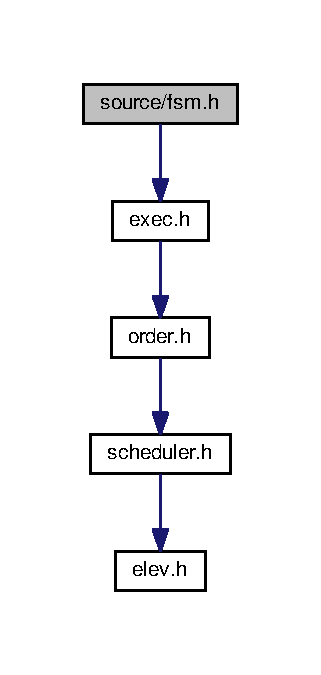
\includegraphics[width=154pt]{fsm_8h__incl}
\end{center}
\end{figure}
This graph shows which files directly or indirectly include this file\+:\nopagebreak
\begin{figure}[H]
\begin{center}
\leavevmode
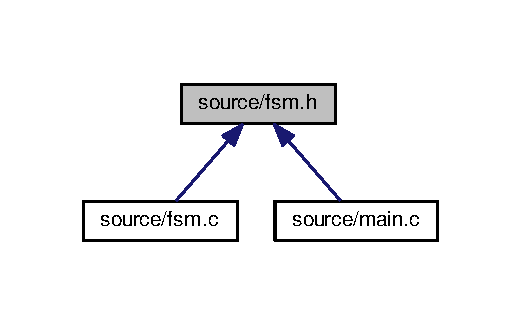
\includegraphics[width=250pt]{fsm_8h__dep__incl}
\end{center}
\end{figure}
\subsection*{Data Structures}
\begin{DoxyCompactItemize}
\item 
struct \hyperlink{structtransition}{transition}
\end{DoxyCompactItemize}
\subsection*{Typedefs}
\begin{DoxyCompactItemize}
\item 
typedef enum state\+\_\+codes {\bfseries state\+\_\+codes\+\_\+t}\hypertarget{fsm_8h_a24468ac18da8c9095490b17865df4fdd}{}\label{fsm_8h_a24468ac18da8c9095490b17865df4fdd}

\item 
typedef struct \hyperlink{structtransition}{transition} {\bfseries transition\+\_\+t}\hypertarget{fsm_8h_a71f0b08ca21f15895e4dff5ea4d2a69e}{}\label{fsm_8h_a71f0b08ca21f15895e4dff5ea4d2a69e}

\end{DoxyCompactItemize}
\subsection*{Enumerations}
\begin{DoxyCompactItemize}
\item 
enum {\bfseries state\+\_\+codes} \{ \\*
{\bfseries floor\+\_\+stationary}, 
{\bfseries initialize}, 
{\bfseries driving\+\_\+up}, 
{\bfseries driving\+\_\+down}, 
\\*
{\bfseries stop\+\_\+state}, 
{\bfseries idle\+\_\+state}, 
{\bfseries end}
 \}\hypertarget{fsm_8h_ab44f81e9f0b8e5687ca7a45c0301d751}{}\label{fsm_8h_ab44f81e9f0b8e5687ca7a45c0301d751}

\end{DoxyCompactItemize}
\subsection*{Functions}
\begin{DoxyCompactItemize}
\item 
return\+\_\+codes\+\_\+t \hyperlink{fsm_8h_acab6b1a742dfe51fcc78f99f24f6c4be}{fsm\+\_\+floor\+\_\+stationary\+\_\+state} (void)
\begin{DoxyCompactList}\small\item\em Algorithm for the stationary state. Listen for orders and return a return code to use in the {\ttfamily lookup\+\_\+transitions} function. \end{DoxyCompactList}\item 
return\+\_\+codes\+\_\+t \hyperlink{fsm_8h_ae67daff4b8088c370b9925d948a8f641}{fsm\+\_\+initialize\+\_\+state} (void)
\begin{DoxyCompactList}\small\item\em Algorithm for the initialization state. Ignore all orders and move down until detects a floor, then stops and returns a return code to use in the {\ttfamily lookup\+\_\+transitions} function. \end{DoxyCompactList}\item 
return\+\_\+codes\+\_\+t \hyperlink{fsm_8h_a6add83788caf3078462c94ce0d46fa92}{fsm\+\_\+driving\+\_\+up\+\_\+state} (void)
\begin{DoxyCompactList}\small\item\em Algorithm for the driving up state. Listen for orders and stop button and return a return code to use in the {\ttfamily lookup\+\_\+transitions} function. \end{DoxyCompactList}\item 
return\+\_\+codes\+\_\+t \hyperlink{fsm_8h_a88e991035ea2a1060d380cc2e4eb6f99}{fsm\+\_\+driving\+\_\+down\+\_\+state} (void)
\begin{DoxyCompactList}\small\item\em Algorithm for the driving down state. Listen for orders and stop button and return a return code to use in the {\ttfamily lookup\+\_\+transitions} function. \end{DoxyCompactList}\item 
return\+\_\+codes\+\_\+t \hyperlink{fsm_8h_a2ec996fa49f353c5a23a0e5c8cf43a1e}{fsm\+\_\+stop\+\_\+state} (void)
\begin{DoxyCompactList}\small\item\em Algorithm fot the stop state. Delete all orders, ignore new orders and stay in stop state while order\+\_\+button is pressed. If stops on floor, keep door open while in this state. When stop button released, return a return code to use in the {\ttfamily lookup\+\_\+transitions} function. \end{DoxyCompactList}\item 
return\+\_\+codes\+\_\+t \hyperlink{fsm_8h_aa88c9061cdcde2d7eb26b564bd8576f7}{fsm\+\_\+idle\+\_\+state} (void)
\begin{DoxyCompactList}\small\item\em Algorithm for the idle state. Listen for orders and stop button and update queues if necessary. Stay idle until at least one order is recieved. Return a return code to use in the {\ttfamily lookup\+\_\+transitions} function. \end{DoxyCompactList}\item 
return\+\_\+codes\+\_\+t \hyperlink{fsm_8h_a4c5d9f64350a9372bdbc476cf735b716}{fsm\+\_\+end\+\_\+state} (void)
\begin{DoxyCompactList}\small\item\em A fail state, used for debugging. \end{DoxyCompactList}\item 
state\+\_\+codes\+\_\+t \hyperlink{fsm_8h_a384346766d6529bb78eac9dcae296ce6}{lookup\+\_\+transitions} (state\+\_\+codes\+\_\+t cur\+\_\+state, return\+\_\+codes\+\_\+t ret\+\_\+code)
\begin{DoxyCompactList}\small\item\em Takes in the current state and a return code generated from the fsm function of that state. Searches through a {\ttfamily state\+\_\+transitions} array which contains all transition combinations and looks for the appropriate one to return a new state code. \end{DoxyCompactList}\end{DoxyCompactItemize}
\subsection*{Variables}
\begin{DoxyCompactItemize}
\item 
return\+\_\+codes\+\_\+t($\ast$ \hyperlink{fsm_8h_a6964675fd0305f58a977292430d9589b}{state} \mbox{[}$\,$\mbox{]})(void)
\item 
\hyperlink{structtransition}{transition\+\_\+t} {\bfseries state\+\_\+transitions} \mbox{[}$\,$\mbox{]}\hypertarget{fsm_8h_ab95c359f41693d31cdbb3c7d46cc08cb}{}\label{fsm_8h_ab95c359f41693d31cdbb3c7d46cc08cb}

\end{DoxyCompactItemize}


\subsection{Detailed Description}
A state machine library. 



\subsection{Function Documentation}
\index{fsm.\+h@{fsm.\+h}!fsm\+\_\+driving\+\_\+down\+\_\+state@{fsm\+\_\+driving\+\_\+down\+\_\+state}}
\index{fsm\+\_\+driving\+\_\+down\+\_\+state@{fsm\+\_\+driving\+\_\+down\+\_\+state}!fsm.\+h@{fsm.\+h}}
\subsubsection[{\texorpdfstring{fsm\+\_\+driving\+\_\+down\+\_\+state(void)}{fsm_driving_down_state(void)}}]{\setlength{\rightskip}{0pt plus 5cm}return\+\_\+codes\+\_\+t fsm\+\_\+driving\+\_\+down\+\_\+state (
\begin{DoxyParamCaption}
\item[{void}]{}
\end{DoxyParamCaption}
)}\hypertarget{fsm_8h_a88e991035ea2a1060d380cc2e4eb6f99}{}\label{fsm_8h_a88e991035ea2a1060d380cc2e4eb6f99}


Algorithm for the driving down state. Listen for orders and stop button and return a return code to use in the {\ttfamily lookup\+\_\+transitions} function. 

\begin{DoxyReturn}{Returns}
Return code of type {\ttfamily return\+\_\+codes\+\_\+t} to find next state. 
\end{DoxyReturn}


Definition at line 189 of file fsm.\+c.

\index{fsm.\+h@{fsm.\+h}!fsm\+\_\+driving\+\_\+up\+\_\+state@{fsm\+\_\+driving\+\_\+up\+\_\+state}}
\index{fsm\+\_\+driving\+\_\+up\+\_\+state@{fsm\+\_\+driving\+\_\+up\+\_\+state}!fsm.\+h@{fsm.\+h}}
\subsubsection[{\texorpdfstring{fsm\+\_\+driving\+\_\+up\+\_\+state(void)}{fsm_driving_up_state(void)}}]{\setlength{\rightskip}{0pt plus 5cm}return\+\_\+codes\+\_\+t fsm\+\_\+driving\+\_\+up\+\_\+state (
\begin{DoxyParamCaption}
\item[{void}]{}
\end{DoxyParamCaption}
)}\hypertarget{fsm_8h_a6add83788caf3078462c94ce0d46fa92}{}\label{fsm_8h_a6add83788caf3078462c94ce0d46fa92}


Algorithm for the driving up state. Listen for orders and stop button and return a return code to use in the {\ttfamily lookup\+\_\+transitions} function. 

\begin{DoxyReturn}{Returns}
Return code of type {\ttfamily return\+\_\+codes\+\_\+t} to find next state. 
\end{DoxyReturn}


Definition at line 150 of file fsm.\+c.

\index{fsm.\+h@{fsm.\+h}!fsm\+\_\+end\+\_\+state@{fsm\+\_\+end\+\_\+state}}
\index{fsm\+\_\+end\+\_\+state@{fsm\+\_\+end\+\_\+state}!fsm.\+h@{fsm.\+h}}
\subsubsection[{\texorpdfstring{fsm\+\_\+end\+\_\+state(void)}{fsm_end_state(void)}}]{\setlength{\rightskip}{0pt plus 5cm}return\+\_\+codes\+\_\+t fsm\+\_\+end\+\_\+state (
\begin{DoxyParamCaption}
\item[{void}]{}
\end{DoxyParamCaption}
)}\hypertarget{fsm_8h_a4c5d9f64350a9372bdbc476cf735b716}{}\label{fsm_8h_a4c5d9f64350a9372bdbc476cf735b716}


A fail state, used for debugging. 

\begin{DoxyReturn}{Returns}
Program exitis before any return occurs.
\end{DoxyReturn}
\begin{DoxyWarning}{Warning}
Elevator should not reach this state, and can not leave it. If it is reached, the program exits with error code {\ttfamily 1}. 
\end{DoxyWarning}


Definition at line 303 of file fsm.\+c.

\index{fsm.\+h@{fsm.\+h}!fsm\+\_\+floor\+\_\+stationary\+\_\+state@{fsm\+\_\+floor\+\_\+stationary\+\_\+state}}
\index{fsm\+\_\+floor\+\_\+stationary\+\_\+state@{fsm\+\_\+floor\+\_\+stationary\+\_\+state}!fsm.\+h@{fsm.\+h}}
\subsubsection[{\texorpdfstring{fsm\+\_\+floor\+\_\+stationary\+\_\+state(void)}{fsm_floor_stationary_state(void)}}]{\setlength{\rightskip}{0pt plus 5cm}return\+\_\+codes\+\_\+t fsm\+\_\+floor\+\_\+stationary\+\_\+state (
\begin{DoxyParamCaption}
\item[{void}]{}
\end{DoxyParamCaption}
)}\hypertarget{fsm_8h_acab6b1a742dfe51fcc78f99f24f6c4be}{}\label{fsm_8h_acab6b1a742dfe51fcc78f99f24f6c4be}


Algorithm for the stationary state. Listen for orders and return a return code to use in the {\ttfamily lookup\+\_\+transitions} function. 

\begin{DoxyReturn}{Returns}
Return code of type {\ttfamily return\+\_\+codes\+\_\+t} to find next state. 
\end{DoxyReturn}


Definition at line 95 of file fsm.\+c.

\index{fsm.\+h@{fsm.\+h}!fsm\+\_\+idle\+\_\+state@{fsm\+\_\+idle\+\_\+state}}
\index{fsm\+\_\+idle\+\_\+state@{fsm\+\_\+idle\+\_\+state}!fsm.\+h@{fsm.\+h}}
\subsubsection[{\texorpdfstring{fsm\+\_\+idle\+\_\+state(void)}{fsm_idle_state(void)}}]{\setlength{\rightskip}{0pt plus 5cm}return\+\_\+codes\+\_\+t fsm\+\_\+idle\+\_\+state (
\begin{DoxyParamCaption}
\item[{void}]{}
\end{DoxyParamCaption}
)}\hypertarget{fsm_8h_aa88c9061cdcde2d7eb26b564bd8576f7}{}\label{fsm_8h_aa88c9061cdcde2d7eb26b564bd8576f7}


Algorithm for the idle state. Listen for orders and stop button and update queues if necessary. Stay idle until at least one order is recieved. Return a return code to use in the {\ttfamily lookup\+\_\+transitions} function. 

\begin{DoxyReturn}{Returns}
Return code of type {\ttfamily return\+\_\+codes\+\_\+t} to find next state. 
\end{DoxyReturn}


Definition at line 279 of file fsm.\+c.

\index{fsm.\+h@{fsm.\+h}!fsm\+\_\+initialize\+\_\+state@{fsm\+\_\+initialize\+\_\+state}}
\index{fsm\+\_\+initialize\+\_\+state@{fsm\+\_\+initialize\+\_\+state}!fsm.\+h@{fsm.\+h}}
\subsubsection[{\texorpdfstring{fsm\+\_\+initialize\+\_\+state(void)}{fsm_initialize_state(void)}}]{\setlength{\rightskip}{0pt plus 5cm}return\+\_\+codes\+\_\+t fsm\+\_\+initialize\+\_\+state (
\begin{DoxyParamCaption}
\item[{void}]{}
\end{DoxyParamCaption}
)}\hypertarget{fsm_8h_ae67daff4b8088c370b9925d948a8f641}{}\label{fsm_8h_ae67daff4b8088c370b9925d948a8f641}


Algorithm for the initialization state. Ignore all orders and move down until detects a floor, then stops and returns a return code to use in the {\ttfamily lookup\+\_\+transitions} function. 

\begin{DoxyReturn}{Returns}
Return code of type {\ttfamily return\+\_\+codes\+\_\+t} to find next state. 
\end{DoxyReturn}


Definition at line 75 of file fsm.\+c.

\index{fsm.\+h@{fsm.\+h}!fsm\+\_\+stop\+\_\+state@{fsm\+\_\+stop\+\_\+state}}
\index{fsm\+\_\+stop\+\_\+state@{fsm\+\_\+stop\+\_\+state}!fsm.\+h@{fsm.\+h}}
\subsubsection[{\texorpdfstring{fsm\+\_\+stop\+\_\+state(void)}{fsm_stop_state(void)}}]{\setlength{\rightskip}{0pt plus 5cm}return\+\_\+codes\+\_\+t fsm\+\_\+stop\+\_\+state (
\begin{DoxyParamCaption}
\item[{void}]{}
\end{DoxyParamCaption}
)}\hypertarget{fsm_8h_a2ec996fa49f353c5a23a0e5c8cf43a1e}{}\label{fsm_8h_a2ec996fa49f353c5a23a0e5c8cf43a1e}


Algorithm fot the stop state. Delete all orders, ignore new orders and stay in stop state while order\+\_\+button is pressed. If stops on floor, keep door open while in this state. When stop button released, return a return code to use in the {\ttfamily lookup\+\_\+transitions} function. 

\begin{DoxyReturn}{Returns}
Return code of type {\ttfamily return\+\_\+codes\+\_\+t} to find next state. 
\end{DoxyReturn}


Definition at line 228 of file fsm.\+c.

\index{fsm.\+h@{fsm.\+h}!lookup\+\_\+transitions@{lookup\+\_\+transitions}}
\index{lookup\+\_\+transitions@{lookup\+\_\+transitions}!fsm.\+h@{fsm.\+h}}
\subsubsection[{\texorpdfstring{lookup\+\_\+transitions(state\+\_\+codes\+\_\+t cur\+\_\+state, return\+\_\+codes\+\_\+t ret\+\_\+code)}{lookup_transitions(state_codes_t cur_state, return_codes_t ret_code)}}]{\setlength{\rightskip}{0pt plus 5cm}state\+\_\+codes\+\_\+t lookup\+\_\+transitions (
\begin{DoxyParamCaption}
\item[{state\+\_\+codes\+\_\+t}]{cur\+\_\+state, }
\item[{return\+\_\+codes\+\_\+t}]{ret\+\_\+code}
\end{DoxyParamCaption}
)}\hypertarget{fsm_8h_a384346766d6529bb78eac9dcae296ce6}{}\label{fsm_8h_a384346766d6529bb78eac9dcae296ce6}


Takes in the current state and a return code generated from the fsm function of that state. Searches through a {\ttfamily state\+\_\+transitions} array which contains all transition combinations and looks for the appropriate one to return a new state code. 


\begin{DoxyParams}[1]{Parameters}
\mbox{\tt in}  & {\em cur\+\_\+state} & The current state the fsm is in. \\
\hline
\mbox{\tt in}  & {\em ret\+\_\+code} & The Return code from the respective fsm state function.\\
\hline
\end{DoxyParams}
\begin{DoxyReturn}{Returns}
Return state code for the next state. 
\end{DoxyReturn}


Definition at line 61 of file fsm.\+c.



\subsection{Variable Documentation}
\index{fsm.\+h@{fsm.\+h}!state@{state}}
\index{state@{state}!fsm.\+h@{fsm.\+h}}
\subsubsection[{\texorpdfstring{state}{state}}]{\setlength{\rightskip}{0pt plus 5cm}return\+\_\+codes\+\_\+t($\ast$  state\mbox{[}$\,$\mbox{]})(void)}\hypertarget{fsm_8h_a6964675fd0305f58a977292430d9589b}{}\label{fsm_8h_a6964675fd0305f58a977292430d9589b}
\begin{DoxyWarning}{Warning}
Must be in sync with {\ttfamily state\+\_\+codes\+\_\+t} 
\end{DoxyWarning}


Definition at line 16 of file fsm.\+c.


\hypertarget{order_8h}{}\section{source/order.h File Reference}
\label{order_8h}\index{source/order.\+h@{source/order.\+h}}


A library for adding and deleting orders in the queues and to fetch the queues themselves.  


{\ttfamily \#include \char`\"{}scheduler.\+h\char`\"{}}\\*
{\ttfamily \#include \char`\"{}fsm.\+h\char`\"{}}\\*
{\ttfamily \#include \char`\"{}elev.\+h\char`\"{}}\\*
Include dependency graph for order.\+h\+:\nopagebreak
\begin{figure}[H]
\begin{center}
\leavevmode
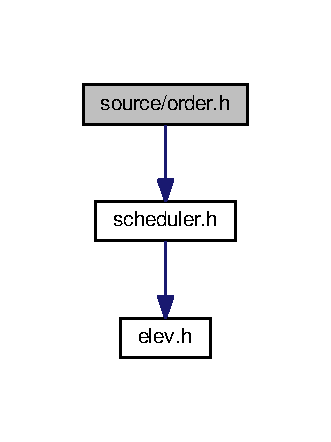
\includegraphics[width=203pt]{order_8h__incl}
\end{center}
\end{figure}
This graph shows which files directly or indirectly include this file\+:\nopagebreak
\begin{figure}[H]
\begin{center}
\leavevmode
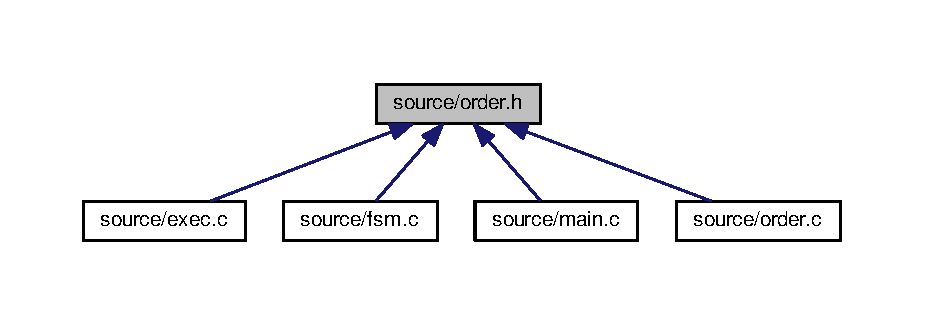
\includegraphics[width=350pt]{order_8h__dep__incl}
\end{center}
\end{figure}
\subsection*{Functions}
\begin{DoxyCompactItemize}
\item 
\hyperlink{structinside__order__queue}{inside\+\_\+queue\+\_\+t} $\ast$ {\bfseries order\+\_\+get\+\_\+inside\+\_\+queue} (void)\hypertarget{order_8h_a211c9e4b31501cbeb31532f649a33b60}{}\label{order_8h_a211c9e4b31501cbeb31532f649a33b60}

\item 
\hyperlink{structoutside__order__queue}{outside\+\_\+queue\+\_\+t} $\ast$ {\bfseries order\+\_\+get\+\_\+outside\+\_\+queue} (void)\hypertarget{order_8h_ac44243f8b378f08f2a9512bba4f75807}{}\label{order_8h_ac44243f8b378f08f2a9512bba4f75807}

\item 
int \hyperlink{order_8h_a6fa2ab20cc3a0f2083a49ca7aada6677}{order\+\_\+add\+\_\+order\+\_\+to\+\_\+queue} (floor\+\_\+codes\+\_\+t floor, elev\+\_\+motor\+\_\+direction\+\_\+t direction)
\begin{DoxyCompactList}\small\item\em Add order to a queue. \end{DoxyCompactList}\item 
void \hyperlink{order_8h_a07b76875e3c2e8f1a8d7884db2a8f91f}{order\+\_\+remove\+\_\+all\+\_\+orders\+\_\+at\+\_\+floor} (floor\+\_\+codes\+\_\+t floor)
\begin{DoxyCompactList}\small\item\em Remove all orders on a given floor from the queues. \end{DoxyCompactList}\item 
void \hyperlink{order_8h_a924d88629bd3a222aed6c74b5f370169}{order\+\_\+remove\+\_\+all\+\_\+orders} ()\hypertarget{order_8h_a924d88629bd3a222aed6c74b5f370169}{}\label{order_8h_a924d88629bd3a222aed6c74b5f370169}

\begin{DoxyCompactList}\small\item\em Remove all orders on all floors from the queues. \end{DoxyCompactList}\item 
void \hyperlink{order_8h_a4bcc1525f84c72fff33601b0a367f39a}{order\+\_\+print\+\_\+orders} ()\hypertarget{order_8h_a4bcc1525f84c72fff33601b0a367f39a}{}\label{order_8h_a4bcc1525f84c72fff33601b0a367f39a}

\begin{DoxyCompactList}\small\item\em Print both queues in a nice and readable format. \end{DoxyCompactList}\end{DoxyCompactItemize}


\subsection{Detailed Description}
A library for adding and deleting orders in the queues and to fetch the queues themselves. 



\subsection{Function Documentation}
\index{order.\+h@{order.\+h}!order\+\_\+add\+\_\+order\+\_\+to\+\_\+queue@{order\+\_\+add\+\_\+order\+\_\+to\+\_\+queue}}
\index{order\+\_\+add\+\_\+order\+\_\+to\+\_\+queue@{order\+\_\+add\+\_\+order\+\_\+to\+\_\+queue}!order.\+h@{order.\+h}}
\subsubsection[{\texorpdfstring{order\+\_\+add\+\_\+order\+\_\+to\+\_\+queue(floor\+\_\+codes\+\_\+t floor, elev\+\_\+motor\+\_\+direction\+\_\+t direction)}{order_add_order_to_queue(floor_codes_t floor, elev_motor_direction_t direction)}}]{\setlength{\rightskip}{0pt plus 5cm}int order\+\_\+add\+\_\+order\+\_\+to\+\_\+queue (
\begin{DoxyParamCaption}
\item[{floor\+\_\+codes\+\_\+t}]{floor, }
\item[{elev\+\_\+motor\+\_\+direction\+\_\+t}]{direction}
\end{DoxyParamCaption}
)}\hypertarget{order_8h_a6fa2ab20cc3a0f2083a49ca7aada6677}{}\label{order_8h_a6fa2ab20cc3a0f2083a49ca7aada6677}


Add order to a queue. 


\begin{DoxyParams}[1]{Parameters}
\mbox{\tt in}  & {\em floor} & Floor Code \\
\hline
\mbox{\tt in}  & {\em direction} & Direction Code\\
\hline
\end{DoxyParams}
\begin{DoxyReturn}{Returns}
0 if order was successfully added to one of the queues, -\/1 if not. 
\end{DoxyReturn}


Definition at line 26 of file order.\+c.

\index{order.\+h@{order.\+h}!order\+\_\+remove\+\_\+all\+\_\+orders\+\_\+at\+\_\+floor@{order\+\_\+remove\+\_\+all\+\_\+orders\+\_\+at\+\_\+floor}}
\index{order\+\_\+remove\+\_\+all\+\_\+orders\+\_\+at\+\_\+floor@{order\+\_\+remove\+\_\+all\+\_\+orders\+\_\+at\+\_\+floor}!order.\+h@{order.\+h}}
\subsubsection[{\texorpdfstring{order\+\_\+remove\+\_\+all\+\_\+orders\+\_\+at\+\_\+floor(floor\+\_\+codes\+\_\+t floor)}{order_remove_all_orders_at_floor(floor_codes_t floor)}}]{\setlength{\rightskip}{0pt plus 5cm}void order\+\_\+remove\+\_\+all\+\_\+orders\+\_\+at\+\_\+floor (
\begin{DoxyParamCaption}
\item[{floor\+\_\+codes\+\_\+t}]{floor}
\end{DoxyParamCaption}
)}\hypertarget{order_8h_a07b76875e3c2e8f1a8d7884db2a8f91f}{}\label{order_8h_a07b76875e3c2e8f1a8d7884db2a8f91f}


Remove all orders on a given floor from the queues. 


\begin{DoxyParams}[1]{Parameters}
\mbox{\tt in}  & {\em floor} & The floor to delete all orders from \\
\hline
\end{DoxyParams}


Definition at line 41 of file order.\+c.


\hypertarget{scheduler_8h}{}\section{source/scheduler.h File Reference}
\label{scheduler_8h}\index{source/scheduler.\+h@{source/scheduler.\+h}}


A library for doing operations on queues.  


{\ttfamily \#include \char`\"{}exec.\+h\char`\"{}}\\*
{\ttfamily \#include \char`\"{}elev.\+h\char`\"{}}\\*
Include dependency graph for scheduler.\+h\+:
% FIG 0
This graph shows which files directly or indirectly include this file\+:
% FIG 1
\subsection*{Data Structures}
\begin{DoxyCompactItemize}
\item 
struct \hyperlink{structinside__order}{inside\+\_\+order}
\item 
struct \hyperlink{structoutside__order}{outside\+\_\+order}
\item 
struct \hyperlink{structinside__order__queue}{inside\+\_\+order\+\_\+queue}
\item 
struct \hyperlink{structoutside__order__queue}{outside\+\_\+order\+\_\+queue}
\end{DoxyCompactItemize}
\subsection*{Macros}
\begin{DoxyCompactItemize}
\item 
\#define {\bfseries M\+A\+X\+\_\+\+I\+N\+S\+I\+D\+E\+\_\+\+O\+R\+D\+E\+RS}~4\hypertarget{scheduler_8h_a0dd4a2af1b76fab4e0ae51d1f915b6cd}{}\label{scheduler_8h_a0dd4a2af1b76fab4e0ae51d1f915b6cd}

\item 
\#define {\bfseries M\+A\+X\+\_\+\+O\+U\+T\+S\+I\+D\+E\+\_\+\+O\+R\+D\+E\+RS}~6\hypertarget{scheduler_8h_a58308d5b99cb9e12b0b5bc385a32a051}{}\label{scheduler_8h_a58308d5b99cb9e12b0b5bc385a32a051}

\end{DoxyCompactItemize}
\subsection*{Typedefs}
\begin{DoxyCompactItemize}
\item 
typedef struct \hyperlink{structinside__order}{inside\+\_\+order} {\bfseries inside\+\_\+order\+\_\+t}\hypertarget{scheduler_8h_a2e78bc07a4b5862db04324b34a40edac}{}\label{scheduler_8h_a2e78bc07a4b5862db04324b34a40edac}

\item 
typedef struct \hyperlink{structoutside__order}{outside\+\_\+order} {\bfseries outside\+\_\+order\+\_\+t}\hypertarget{scheduler_8h_afd3fb63c53d1ff17ed6dd184ae2d2f2f}{}\label{scheduler_8h_afd3fb63c53d1ff17ed6dd184ae2d2f2f}

\item 
typedef struct \hyperlink{structinside__order__queue}{inside\+\_\+order\+\_\+queue} {\bfseries inside\+\_\+queue\+\_\+t}\hypertarget{scheduler_8h_a17f3c53e316d7009188e19e4efd3091e}{}\label{scheduler_8h_a17f3c53e316d7009188e19e4efd3091e}

\item 
typedef struct \hyperlink{structoutside__order__queue}{outside\+\_\+order\+\_\+queue} {\bfseries outside\+\_\+queue\+\_\+t}\hypertarget{scheduler_8h_a514ed46871c432efe1b157d3cc64114a}{}\label{scheduler_8h_a514ed46871c432efe1b157d3cc64114a}

\end{DoxyCompactItemize}
\subsection*{Functions}
\begin{DoxyCompactItemize}
\item 
void \hyperlink{scheduler_8h_ab5dfe0c4039ae459a9caca4e8274567c}{scheduler\+\_\+insert\+\_\+inside\+\_\+order} (\hyperlink{structinside__order__queue}{inside\+\_\+queue\+\_\+t} $\ast$queue, floor\+\_\+codes\+\_\+t floor)
\begin{DoxyCompactList}\small\item\em Insert an order into an inside queue for orders made inside the elevator. \end{DoxyCompactList}\item 
void \hyperlink{scheduler_8h_a7fc902a584b4324118bd9a6a1039c971}{scheduler\+\_\+delete\+\_\+inside\+\_\+order} (\hyperlink{structinside__order__queue}{inside\+\_\+queue\+\_\+t} $\ast$queue, floor\+\_\+codes\+\_\+t floor)
\begin{DoxyCompactList}\small\item\em Delete an order from an inside queue for orders made inside the elevator. \end{DoxyCompactList}\item 
void \hyperlink{scheduler_8h_a5fc45e58536832d318435377fa3bd3e2}{scheduler\+\_\+display\+\_\+inside\+\_\+queue} (\hyperlink{structinside__order__queue}{inside\+\_\+queue\+\_\+t} $\ast$queue)
\begin{DoxyCompactList}\small\item\em Prints an inside queue for orders made inside the elevator. \end{DoxyCompactList}\item 
void \hyperlink{scheduler_8h_a0a5628c59ff448a29f3c44e329591bf9}{scheduler\+\_\+insert\+\_\+outside\+\_\+order} (\hyperlink{structoutside__order__queue}{outside\+\_\+queue\+\_\+t} $\ast$queue, floor\+\_\+codes\+\_\+t floor, elev\+\_\+motor\+\_\+direction\+\_\+t direction)
\begin{DoxyCompactList}\small\item\em Insert an order into an outside queue for orders made outside of the elevator. \end{DoxyCompactList}\item 
void \hyperlink{scheduler_8h_a893ecb3f677e664b942585482edee04c}{scheduler\+\_\+delete\+\_\+outside\+\_\+order} (\hyperlink{structoutside__order__queue}{outside\+\_\+queue\+\_\+t} $\ast$queue, floor\+\_\+codes\+\_\+t floor, elev\+\_\+motor\+\_\+direction\+\_\+t direction)
\begin{DoxyCompactList}\small\item\em Delete an order in an outside queue for orders made outside of the elevator. \end{DoxyCompactList}\item 
void \hyperlink{scheduler_8h_abc0eaafc54d6666879332ed0f99096c6}{scheduler\+\_\+display\+\_\+outside\+\_\+queue} (\hyperlink{structoutside__order__queue}{outside\+\_\+queue\+\_\+t} $\ast$queue)
\begin{DoxyCompactList}\small\item\em Prints an outside queue for orders made outside the elevator. \end{DoxyCompactList}\end{DoxyCompactItemize}


\subsection{Detailed Description}
A library for doing operations on queues. 



\subsection{Function Documentation}
\index{scheduler.\+h@{scheduler.\+h}!scheduler\+\_\+delete\+\_\+inside\+\_\+order@{scheduler\+\_\+delete\+\_\+inside\+\_\+order}}
\index{scheduler\+\_\+delete\+\_\+inside\+\_\+order@{scheduler\+\_\+delete\+\_\+inside\+\_\+order}!scheduler.\+h@{scheduler.\+h}}
\subsubsection[{\texorpdfstring{scheduler\+\_\+delete\+\_\+inside\+\_\+order(inside\+\_\+queue\+\_\+t $\ast$queue, floor\+\_\+codes\+\_\+t floor)}{scheduler_delete_inside_order(inside_queue_t *queue, floor_codes_t floor)}}]{\setlength{\rightskip}{0pt plus 5cm}void scheduler\+\_\+delete\+\_\+inside\+\_\+order (
\begin{DoxyParamCaption}
\item[{{\bf inside\+\_\+queue\+\_\+t} $\ast$}]{queue, }
\item[{floor\+\_\+codes\+\_\+t}]{floor}
\end{DoxyParamCaption}
)}\hypertarget{scheduler_8h_a7fc902a584b4324118bd9a6a1039c971}{}\label{scheduler_8h_a7fc902a584b4324118bd9a6a1039c971}


Delete an order from an inside queue for orders made inside the elevator. 


\begin{DoxyParams}[1]{Parameters}
\mbox{\tt out}  & {\em queue} & Buffer queue \\
\hline
\mbox{\tt in}  & {\em floor} & Order floor \\
\hline
\end{DoxyParams}


Definition at line 38 of file scheduler.\+c.

\index{scheduler.\+h@{scheduler.\+h}!scheduler\+\_\+delete\+\_\+outside\+\_\+order@{scheduler\+\_\+delete\+\_\+outside\+\_\+order}}
\index{scheduler\+\_\+delete\+\_\+outside\+\_\+order@{scheduler\+\_\+delete\+\_\+outside\+\_\+order}!scheduler.\+h@{scheduler.\+h}}
\subsubsection[{\texorpdfstring{scheduler\+\_\+delete\+\_\+outside\+\_\+order(outside\+\_\+queue\+\_\+t $\ast$queue, floor\+\_\+codes\+\_\+t floor, elev\+\_\+motor\+\_\+direction\+\_\+t direction)}{scheduler_delete_outside_order(outside_queue_t *queue, floor_codes_t floor, elev_motor_direction_t direction)}}]{\setlength{\rightskip}{0pt plus 5cm}void scheduler\+\_\+delete\+\_\+outside\+\_\+order (
\begin{DoxyParamCaption}
\item[{{\bf outside\+\_\+queue\+\_\+t} $\ast$}]{queue, }
\item[{floor\+\_\+codes\+\_\+t}]{floor, }
\item[{elev\+\_\+motor\+\_\+direction\+\_\+t}]{direction}
\end{DoxyParamCaption}
)}\hypertarget{scheduler_8h_a893ecb3f677e664b942585482edee04c}{}\label{scheduler_8h_a893ecb3f677e664b942585482edee04c}


Delete an order in an outside queue for orders made outside of the elevator. 


\begin{DoxyParams}[1]{Parameters}
\mbox{\tt out}  & {\em queue} & Buffer queue \\
\hline
\mbox{\tt in}  & {\em floor} & Order Floor \\
\hline
\mbox{\tt in}  & {\em direction} & Order Direction \\
\hline
\end{DoxyParams}


Definition at line 127 of file scheduler.\+c.

\index{scheduler.\+h@{scheduler.\+h}!scheduler\+\_\+display\+\_\+inside\+\_\+queue@{scheduler\+\_\+display\+\_\+inside\+\_\+queue}}
\index{scheduler\+\_\+display\+\_\+inside\+\_\+queue@{scheduler\+\_\+display\+\_\+inside\+\_\+queue}!scheduler.\+h@{scheduler.\+h}}
\subsubsection[{\texorpdfstring{scheduler\+\_\+display\+\_\+inside\+\_\+queue(inside\+\_\+queue\+\_\+t $\ast$queue)}{scheduler_display_inside_queue(inside_queue_t *queue)}}]{\setlength{\rightskip}{0pt plus 5cm}void scheduler\+\_\+display\+\_\+inside\+\_\+queue (
\begin{DoxyParamCaption}
\item[{{\bf inside\+\_\+queue\+\_\+t} $\ast$}]{queue}
\end{DoxyParamCaption}
)}\hypertarget{scheduler_8h_a5fc45e58536832d318435377fa3bd3e2}{}\label{scheduler_8h_a5fc45e58536832d318435377fa3bd3e2}


Prints an inside queue for orders made inside the elevator. 


\begin{DoxyParams}[1]{Parameters}
\mbox{\tt in}  & {\em queue} & Queue to print \\
\hline
\end{DoxyParams}


Definition at line 71 of file scheduler.\+c.

\index{scheduler.\+h@{scheduler.\+h}!scheduler\+\_\+display\+\_\+outside\+\_\+queue@{scheduler\+\_\+display\+\_\+outside\+\_\+queue}}
\index{scheduler\+\_\+display\+\_\+outside\+\_\+queue@{scheduler\+\_\+display\+\_\+outside\+\_\+queue}!scheduler.\+h@{scheduler.\+h}}
\subsubsection[{\texorpdfstring{scheduler\+\_\+display\+\_\+outside\+\_\+queue(outside\+\_\+queue\+\_\+t $\ast$queue)}{scheduler_display_outside_queue(outside_queue_t *queue)}}]{\setlength{\rightskip}{0pt plus 5cm}void scheduler\+\_\+display\+\_\+outside\+\_\+queue (
\begin{DoxyParamCaption}
\item[{{\bf outside\+\_\+queue\+\_\+t} $\ast$}]{queue}
\end{DoxyParamCaption}
)}\hypertarget{scheduler_8h_abc0eaafc54d6666879332ed0f99096c6}{}\label{scheduler_8h_abc0eaafc54d6666879332ed0f99096c6}


Prints an outside queue for orders made outside the elevator. 


\begin{DoxyParams}[1]{Parameters}
\mbox{\tt in}  & {\em queue} & Queue to print \\
\hline
\end{DoxyParams}


Definition at line 165 of file scheduler.\+c.

\index{scheduler.\+h@{scheduler.\+h}!scheduler\+\_\+insert\+\_\+inside\+\_\+order@{scheduler\+\_\+insert\+\_\+inside\+\_\+order}}
\index{scheduler\+\_\+insert\+\_\+inside\+\_\+order@{scheduler\+\_\+insert\+\_\+inside\+\_\+order}!scheduler.\+h@{scheduler.\+h}}
\subsubsection[{\texorpdfstring{scheduler\+\_\+insert\+\_\+inside\+\_\+order(inside\+\_\+queue\+\_\+t $\ast$queue, floor\+\_\+codes\+\_\+t floor)}{scheduler_insert_inside_order(inside_queue_t *queue, floor_codes_t floor)}}]{\setlength{\rightskip}{0pt plus 5cm}void scheduler\+\_\+insert\+\_\+inside\+\_\+order (
\begin{DoxyParamCaption}
\item[{{\bf inside\+\_\+queue\+\_\+t} $\ast$}]{queue, }
\item[{floor\+\_\+codes\+\_\+t}]{floor}
\end{DoxyParamCaption}
)}\hypertarget{scheduler_8h_ab5dfe0c4039ae459a9caca4e8274567c}{}\label{scheduler_8h_ab5dfe0c4039ae459a9caca4e8274567c}


Insert an order into an inside queue for orders made inside the elevator. 


\begin{DoxyParams}[1]{Parameters}
\mbox{\tt out}  & {\em queue} & Buffer queue \\
\hline
\mbox{\tt in}  & {\em floor} & Order floor \\
\hline
\end{DoxyParams}


Definition at line 16 of file scheduler.\+c.

\index{scheduler.\+h@{scheduler.\+h}!scheduler\+\_\+insert\+\_\+outside\+\_\+order@{scheduler\+\_\+insert\+\_\+outside\+\_\+order}}
\index{scheduler\+\_\+insert\+\_\+outside\+\_\+order@{scheduler\+\_\+insert\+\_\+outside\+\_\+order}!scheduler.\+h@{scheduler.\+h}}
\subsubsection[{\texorpdfstring{scheduler\+\_\+insert\+\_\+outside\+\_\+order(outside\+\_\+queue\+\_\+t $\ast$queue, floor\+\_\+codes\+\_\+t floor, elev\+\_\+motor\+\_\+direction\+\_\+t direction)}{scheduler_insert_outside_order(outside_queue_t *queue, floor_codes_t floor, elev_motor_direction_t direction)}}]{\setlength{\rightskip}{0pt plus 5cm}void scheduler\+\_\+insert\+\_\+outside\+\_\+order (
\begin{DoxyParamCaption}
\item[{{\bf outside\+\_\+queue\+\_\+t} $\ast$}]{queue, }
\item[{floor\+\_\+codes\+\_\+t}]{floor, }
\item[{elev\+\_\+motor\+\_\+direction\+\_\+t}]{direction}
\end{DoxyParamCaption}
)}\hypertarget{scheduler_8h_a0a5628c59ff448a29f3c44e329591bf9}{}\label{scheduler_8h_a0a5628c59ff448a29f3c44e329591bf9}


Insert an order into an outside queue for orders made outside of the elevator. 


\begin{DoxyParams}[1]{Parameters}
\mbox{\tt out}  & {\em queue} & Buffer queue \\
\hline
\mbox{\tt in}  & {\em floor} & Order floor \\
\hline
\mbox{\tt in}  & {\em direction} & Order direction \\
\hline
\end{DoxyParams}


Definition at line 91 of file scheduler.\+c.


%--- End generated contents ---

% Index
\backmatter
\newpage
\phantomsection
\clearemptydoublepage
\addcontentsline{toc}{chapter}{Index}
\printindex

\end{document}
